\chapter{DC-DC Converters Modeling}

\section{Buck Converter}

The buck converter circuit is illustrated in \autoref{fig:buck_converter}. In this circuit, $v_{\rm{in}}(t)$ represents the input voltage, and $D$ denotes the diode. The output voltage filter consists of an inductor with winding resistance $R_L$ and inductance $L$, and a capacitor with capacitance $C$. Finally, two types of loads are supplied: a Constant Resistance Load with resistance $R(t)$ and a Constant Power Load (CPL) with power $P_{\ell}(t)$, represented by a controlled current source.

\begin{figure}[h]
  \centering
  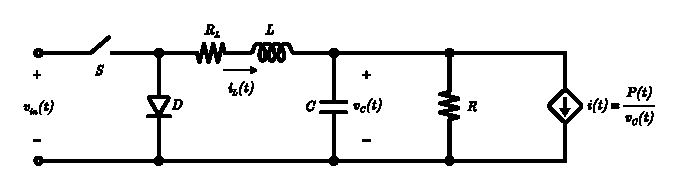
\includegraphics[scale=1.]{figures/buck_converter.eps}
  \caption{Buck converter circuit.}
  \label{fig:buck_converter}
\end{figure}

\subsection{Non-linear Buck Converter Model}

When the switch $S$ is in the off state fot the duration $t_{\rm{off}}$, the dynamic equations describing the circuit's behavior at this moment, derived from Kirchhoff's laws, are as follows:
\begin{equation}
  \begin{cases}
    \dot i_L = - \frac{R_L} L i(t) - \frac{1}{L} v_C(t) \\[8pt]
    \dot v_C = \frac{1}{C} i_L(t) - \frac{1}{C R} v_C(t) - \frac{1}{C v_C(t)} P_{\ell}(t)
  \end{cases}
  \label{eq:buck_state_off}
\end{equation}
And, when the switch $S$ is in the on state for the duration $t_{\rm{on}}$,
\begin{equation}
  \begin{cases}
    \dot i_L = - \frac{R_L} L i(t) - \frac{1}{L} v_C(t) + \frac{1}{L} v_{\rm{in}}(t) \\[8pt]
    \dot v_C = \frac{1}{C} i_L(t) - \frac{1}{C R} v_C(t) - \frac{1}{C v_C(t)} P_{\ell}(t)
  \end{cases}
  \label{eq:buck_state_on}
\end{equation}

Building on the equations \eqref{eq:buck_state_off} and \eqref{eq:buck_state_on}, the average dynamic model that represents the behavior of the buck converter throughout its operation is:
\begin{equation}
  \begin{cases}
    \dot i_L = \left[- \frac{R_L} L i(t) - \frac{1}{L} v_C(t) \right] \frac{t_{\rm{off}}}{t_{\rm{off}} + t_{\rm{on}}} + \left[- \frac{R_L} L i(t) - \frac{1}{L} v_C(t) + \frac{1}{L} v_{\rm{in}}(t)\right] \frac{t_{\rm{on}}}{t_{\rm{off}} + t_{\rm{on}}} \\[8pt]
    \dot v_C = \left[- \frac{1}{C} i_L(t) - \frac{1}{C R} v_C(t) - \frac{1}{C v_C(t)} P_{\ell}(t)\right] \frac{t_{\rm{off}}}{t_{\rm{off}} + t_{\rm{on}}} + \left[- \frac{1}{C} i_L(t) - \frac{1}{C R} v_C(t) - \frac{1}{C v_C(t)} P_{\ell}(t)\right] \frac{t_{\rm{on}}}{t_{\rm{off}} + t_{\rm{on}}}
  \end{cases}
  \label{eq:buck_average_model_1}
\end{equation}

Defining the following expression:
\begin{equation}
  d = \frac{t_{\rm{on}}}{t_{\rm{off}} + t_{\rm{on}}},
\end{equation}
yields,
\begin{equation}
  \frac{t_{\rm{off}} + t_{\rm{on}}}{t_{\rm{off}} + t_{\rm{on}}} = 1 \Rightarrow
  \frac{t_{\rm{off}}}{t_{\rm{off}} + t_{\rm{on}}}
  + \frac{t_{\rm{on}}}{t_{\rm{off}} + t_{\rm{on}}} = 1 \Rightarrow
  \frac{t_{\rm{off}}}{t_{\rm{off}} + t_{\rm{on}}} = 1 - \frac{t_{\rm{on}}}{t_{\rm{off}} + t_{\rm{on}}} \Rightarrow
  \frac{t_{\rm{off}}}{t_{\rm{off}} + t_{\rm{on}}} = 1 - d
\end{equation}

Therefore, the equation \eqref{eq:buck_average_model_1} can be rewritten as follows:
\begin{equation*}
  \begin{cases}
    \dot i_L = \left[- \frac{R_L} L i(t) - \frac{1}{L} v_C(t) \right] \left(1 - d\right) + \left[- \frac{R_L} L i(t) - \frac{1}{L} v_C(t) + \frac{1}{L} v_{\rm{in}}(t)\right] d \\[8pt]
    \dot v_C = \left[- \frac{1}{C} i_L(t) - \frac{1}{C R} v_C(t) - \frac{1}{C v_C(t)} P_{\ell}(t)\right] \left(1 - d\right) + \left[- \frac{1}{C} i_L(t) - \frac{1}{C R} v_C(t) - \frac{1}{C v_C(t)} P_{\ell}(t)\right] d
  \end{cases}
\end{equation*}
Then,
\begin{equation}
  \begin{cases}
    \dot i_L = - \frac{R_L} L i(t) - \frac{1}{L} v_C(t) + \frac{1}{L} v_{\rm{in}}(t) d \\[8pt]
    \dot v_C = - \frac{1}{C} i_L(t) - \frac{1}{C R} v_C(t) - \frac{1}{C v_C(t)} P_{\ell}(t)
  \end{cases}
  \label{eq:buck_conveter_nonlinear_model}
\end{equation}

The variable $d$ is commonly known as the switching duty cycle, which plays a crucial role in controlling switch states. Its value can be determined based on the control input $u_d(t)$, defined by:
\begin{equation}
  d(u_d(t)) = \max\left\{\min\{u_d(t), 1\}, 0\right\}.
\end{equation}
Choosing the operation point $P^{\rm o} = (i_L^{\rm o}, v_C^{\rm o}, u_d^{\rm o}, v_{\rm in}^{\rm o}, P_{\ell}^{\rm o})$, where $u_d^{\rm o} \in \left[0,1\right]$, the following coordinate change can be performed:
\begin{gather}
  \begin{align}
    \delta i_L(t) & = i_L(t) - i_L^{\rm o}, &
    \delta v_C(t) & = v_C(t) - v_C^{\rm o}, &
    \delta u_d(t) & = u_d(t) - u_d^{\rm o}
  \end{align} \\
  \begin{align}
    \delta v_{\rm in}(t) & = v_{\rm in}(t) - v_{\rm in}^{\rm o} &
    \delta P_{\ell}(t)   & = P_{\ell}(t) - P_{\ell}^{\rm o}
  \end{align}
\end{gather}
Moreover, let the control input saturation be modeled by means of the function $\rm{sat} : \mathbb{R} \rightarrow \left[-\upsilon , \upsilon  \right]$ such that:
\begin{gather}
  \delta d = {\rm sat} (\delta u_d(t)) = \max\left\{\min\left\{\delta u_d(t), \upsilon\right\}, -\upsilon\right\} \\
  \upsilon = \min\left\{1 - u_d^{\rm o}, u_d^{\rm o}\right\}
\end{gather}
Thus, the following non-linear model is obtained:
\begin{equation}
  \begin{cases}
    \delta \dot i_L = - \frac{R_L} L \delta i(t) - \frac{1}{L} \delta v_C(t) + \frac{v_{\rm{in}}^{\rm o} +\delta v_{\rm{in}}(t)}{L} {\rm sat}(\delta u_d(t)) + \frac{u_d^{\rm o}}{L} \delta v_{\rm in} (t) \\[8pt]
    \delta \dot v_C = \frac{1}{C} \delta i_L(t) + \left[- \frac{1}{C R}
      + \frac{P_{\ell}^o}{C v_C^o \left[v_C^o + \delta v_C(t)\right]} \right] \delta v_C(t)
    - \frac{1}{C \left[v_C^{\rm o} + \delta v_C(t)\right] } \delta P_{\ell}(t)
  \end{cases}
  \label{eq:buck_conveter_nonlinear_model_sat}
\end{equation}
where, 
\begin{align}
  & \begin{aligned}
      i_L^{\mathrm{o}} & = \frac{1}{R} v_C^{\mathrm{o}} + \frac{1}{v_C^{\mathrm{o}}} P_{\ell}^{\mathrm{o}},
    \end{aligned}
  & \begin{aligned}
      u_d^{\mathrm{o}} & = \frac{R_L}{v_{\mathrm{in}}^{\rm o}} i_L^{\mathrm{o}} + \frac{v_C^{\mathrm{o}}}{v_{\mathrm{in}}^{\rm o}}.
    \end{aligned}
    \notag
\end{align}
Finally, the model \eqref{eq:buck_conveter_nonlinear_model_sat} can be rewritten as:
\begin{equation}
  \dot x = A(x) x(t) + B(w) {\rm sat}(u(t)) + E(x,u) w(t)
  \label{eq:buck_conveter_nonlinear_model_ssm}
\end{equation}
where $x(t) = \begin{bmatrix}i_L(t) & v_C(t)\end{bmatrix}^{\rm{T}}$, $u(t) = \delta u_d(t)$, $w(t) = \begin{bmatrix} \delta v_{\rm in}(t) & \delta P_{\ell}(t)\end{bmatrix}^{\rm{T}}$, and
\begin{gather}
  \notag
  \begin{align}
    A(x) & = \begin{bmatrix}
               - \frac{R_L}{L} & - \frac{1}{L}                                                                   \\[8pt]
               \frac{1}{C}     & - \frac{1}{C R} + \frac{P_{\ell}^o}{C v_C^o \left[v_C^o + \delta v_C(t)\right]}
             \end{bmatrix} &
    B(w) & = \begin{bmatrix}
               \frac{v_{\rm{in}}^{\rm o} +\delta v_{\rm{in}}(t)}{L} \\[8pt] 0
             \end{bmatrix}
  \end{align}
  % \label{eq:buck_conveter_nonlinear_model_ssm_ab} 
  \\[12pt]
  E(x,u) = \begin{bmatrix}
    \frac{u_d^{\rm o}}{L} & 0 \\[8pt] 0 &  - \frac{1}{C \left[v_C^{\rm o} + \delta v_C(t)\right] }
  \end{bmatrix}
  \label{eq:buck_conveter_nonlinear_model_ssm_e}
\end{gather}

\subsection{Buck Converter Fuzzy Model}

In order to address the nonlinearity introduced by saturation, an approach based on substituting ${\rm sat(\circ)}$ with a dead-zone type nonlinearity is used. The dead-zone nonlinearity is defined as:
\begin{equation}
  \psi(u(t)) \triangleq u(t) - {\rm sat}(u(t))
\end{equation}
From the matrices presented in equation \eqref{eq:buck_conveter_nonlinear_model_ssm_e}, it follows $\frac{1}{v_C^{\rm o} + \delta v_C^{\rm o}}$ and $v_{\rm{in}}^{\rm o} +\delta v_{\rm{in}}(t)$ are non-linear terms. For the non-linear terms, are defined
\begin{align}
  z_0(t) & \equiv \frac{1}{v_C^{\rm o} + \delta v_C^{\rm o}}  & \txt{and} &  &
  z_1(t) & \equiv v_{\rm{in}}^{\rm o} +\delta v_{\rm{in}}(t).
\end{align}
Thus, the equation \eqref{eq:buck_conveter_nonlinear_model_ssm} can be rewritten as:
\begin{equation}
  \dot x = A(z(t)) x(t) + B(z(t)) u(t) - B(w) \psi(u(t)) + E(z(t)) w(t),
\end{equation}
where $z(t) = \begin{bmatrix}z_0(t) & z_1(t)\end{bmatrix}$, $A(z(t))  = \begin{bmatrix}
    - \frac{R_L}{L} & - \frac{1}{L}                                       \\[8pt]
    \frac{1}{C}     & - \frac{1}{C R} + \frac{P_{\ell}^o}{C v_C^o} z_0(t)
  \end{bmatrix}$, $B(z(t))  = \begin{bmatrix}
    \frac{1}{L} z_1(t) \\[8pt] 0
  \end{bmatrix}$ and $E(z(t))  = \begin{bmatrix}
    \frac{u_d^{\rm o}}{L} & 0 \\[8pt] 0   & - \frac{1}{C} z_0(t)
  \end{bmatrix}$.

Next, the minimum and maximum values of $z_0(t)$ e $z_1(t)$ under $v_C(t) \in \left[v_C^{\rm{min}}, v_C^{\rm{max}}\right]$ and $v_{\rm{in}}(t) \in \left[v_{\rm{in}}^{\rm{min}}, v_{\rm{in}}^{\rm{max}}\right]$, are obtained as follows:
\begin{equation}
  \begin{cases}
    z_i^0 & = \min\limits_{v_C(t), v_{\rm{in}}(t)} z_i(t) \\[8pt]
    z_i^1 & = \max\limits_{v_C(t), v_{\rm{in}}(t)} z_i(t)
  \end{cases}, \hspace{12pt }i = 1, 2
\end{equation}

From the maximum and minimum values of $z_0(t)$ and $z_1(t)$, the membership functions can be calculated as:
\begin{equation}
  z_i(t) = \sum\limits_{j = 0}^{1} M_i^{j}(z_i(t)) z_i^{j}, \hspace{12pt} \txt{where }
  \hspace{12pt} M_i^1 = \frac{z_i(t) - z_i^0}{z_i^1 - z_i^0} \hspace{8pt} \txt{and} \hspace{8pt}
  M_i^0 = 1 - M_i^1,
  \hspace{12pt} \txt{for} i = \{1,2\}.
\end{equation}

Therefore, the Takagi-Sugeno fuzzy model for the buck converter is:
\begin{equation}
  \dot x = \sum\limits_{i=0}^1 \sum\limits_{j=0}^1 \prod\limits_{k=1}^2 M_k^i(z_k(t))
  \left[
    A\left(z^{\left\{i,j\right\}}\right) x(t) +
    B\left(z^{\left\{i,j\right\}}\right) u(t) -
    B\left(z^{\left\{i,j\right\}}\right) \psi(u(t)) +
    E\left(z^{\left\{i,j\right\}}\right) w(t)
  \right]
  \label{eq:buck_converter_fuzzy_model_summations}
\end{equation}
where $z^{\left\{i,j\right\}}(t)$ is a shorthand for $\begin{bmatrix} z_1^i(t) & z_2^j(t) \end{bmatrix}$.

The summations in \eqref{eq:buck_converter_fuzzy_model_summations} can be aggregated as one summations:
\begin{equation}
  \dot x = \sum\limits_{p=\{0,0\}}^{\{1,1\}} h_p(z(t))
  \left\{A_p x(t) + B_p u(t) - B_p \psi(u(t)) + E_p w(t)\right\}
\end{equation}
where $p = \{b_1, b_2\} \in \mathbb{B}^2$, $\mathbb{B} = \{0,1\}$, 
\begin{gather}
  h_p(z(t)) = \prod\limits_{k=1}^2 M_k^{b_k} (z_k(t)) \\
  \begin{align}
    A_p &= A(z^p) & B_p &= B(z^p) & E_p &= E(z^p)
  \end{align}
\end{gather}
